\section{Experiment 3. 07.02.2020}\label{experiment-3.-07.02.2020}

It took place on 27.02.2020. We aimed to check how \textbf{2 major updates} of the \gls{android} app behave.

The \emph{first} update concerns the usage of \gls{http} requests instead of \gls{mqtt}. We suspected that \gls{mqtt}-protocol is the reason of previously detected issues.

The \emph{second} update is to refactor the source code. It includes switching to \gls{mvvm} architectural pattern, removing of insignificant interface components.

\subsection{Procedure}

Due to the bad weather conditions (heavy snowfall), we decided to perform experiments indoor (Mensa). Mensa is a 2-floor building in TU Ilmenau, it has a large area inside.

The layout included 1 \gls{command_n_center}, 1 \gls{ap}, and 3 \glspl{ue} took part.

All \glspl{ue} can connect to \gls{command_n_center} successfully:

\begin{itemize}
	\tightlist
	\item
	`Push once' button pressed
	\item
	deviceId assigned
	\item
	UE coordinates displayed
\end{itemize}

\subsection{Consideration during the experiment}

As for `Push continuously', it should be known in advance the
coordinates updated on the display \textbf{only in the case of moving to some minimal delta} (10 centimeters). This is insured based on \gls{gnss} values passed by the \gls{android} device.

To make sure the connection is still alive and the values are transferred, we checked the log journal periodically.

\subsection{Outcome}

To sum up, the system finally started working without failures and the meaningful set of data is collected, as shown in the following figures.



\begin{figure}[H]
	\centering
	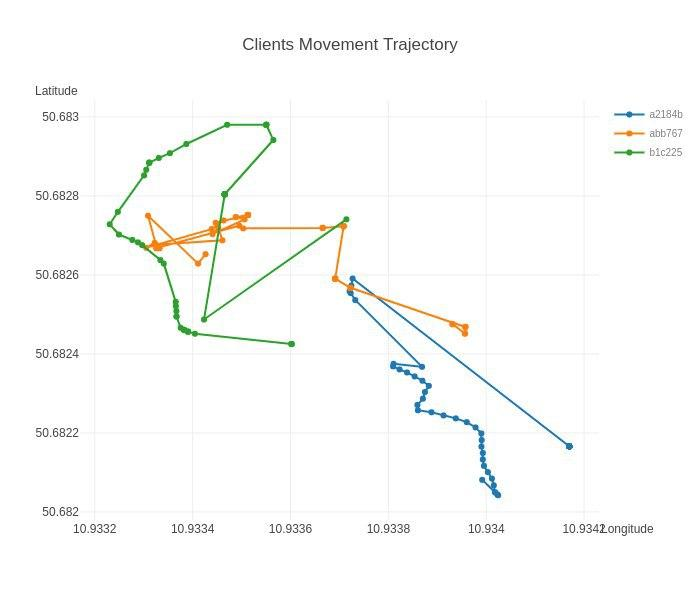
\includegraphics[width=0.5\linewidth,keepaspectratio]{images/experiment_3_1.jpg}
	\caption{Movement trajectory of connected phones}
	\label{fig:movement-trajectory}
\end{figure}

Figure \ref{fig:movement-trajectory} shows movement trajectory of connected clients. 

\begin{figure}[H]
	\centering
	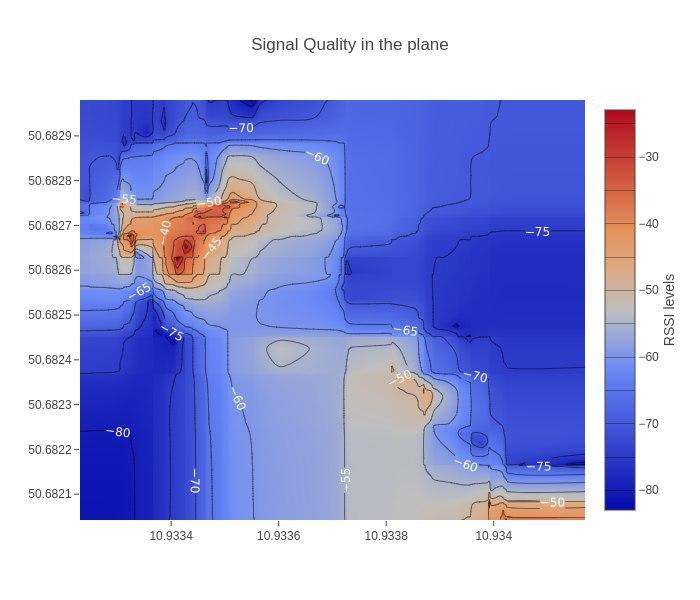
\includegraphics[width=0.5\linewidth,keepaspectratio]{images/experiment_3_2.jpg}
	\caption{Signal quality map}
	\label{fig:signal-quality-heatmap}
\end{figure}

Figure \ref{fig:signal-quality-heatmap} shows how signal changes in different location inside Mensa. Due to obstacles (concrete walls, metal objects), the signal rapidly decreases in the farthest corners and on the second floor.

Figure \ref{fig:signal-quality-changes} describes changes in \acrshort{rss} while \glspl{ue} were moving inside the building. It is clear to observe that some phones started transmitting later than others. If a \gls{ue} fails to send a measurement message, it stores in a local database and resends once the connection is back.


\begin{figure}[H]
	\centering
	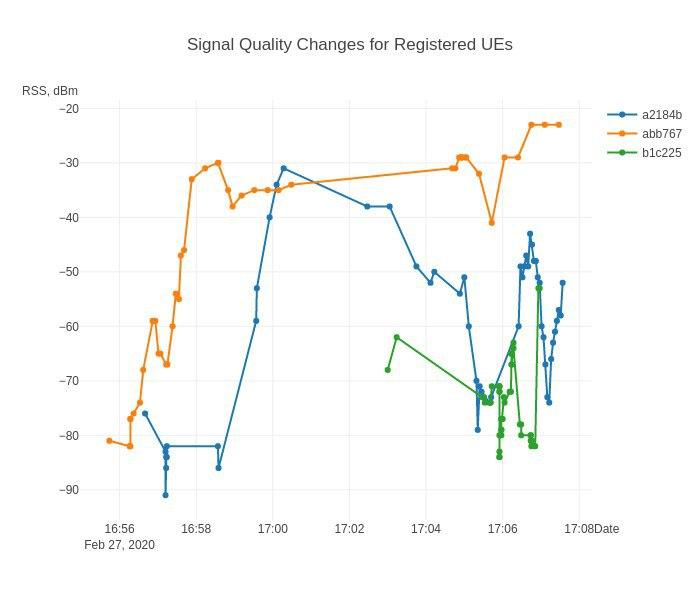
\includegraphics[width=0.5\linewidth,keepaspectratio]{images/experiment_3_3.jpg}
	\caption{Signal quality changes}
	\label{fig:signal-quality-changes}
\end{figure}
